\documentclass[12pt,letterpaper]{article}

\newcommand\hwnumber{C1M3}
\usepackage{fullpage}
\usepackage[top=2cm, bottom=4.5cm, left=2.5cm, right=2.5cm]{geometry}
\usepackage{amsmath,amsthm,amsfonts,amssymb,amscd}
\usepackage{lastpage}
\usepackage{enumerate}
\usepackage{fancyhdr}
\usepackage{mathrsfs}
\usepackage{xcolor}
\usepackage{graphicx}
\usepackage{listings}
\usepackage{hyperref}
\usepackage{enumitem}


\hypersetup{%
  colorlinks=true,
  linkcolor=blue,
  linkbordercolor={0 0 1}
}
% Reduce whitespace around figures
\setlength\intextsep{0pt}
 
 \newcommand{\twolines}{\vspace{5em}}
 \newcommand{\smallspace}{\vspace{12em}}
 \newcommand{\bigspace}{\vspace{60em}}
 
\renewcommand\lstlistingname{Algorithm}
\renewcommand\lstlistlistingname{Algorithms}
\def\lstlistingautorefname{Alg.}

\lstdefinestyle{Python}{
    language        = Python,
    frame           = lines, 
    basicstyle      = \footnotesize,
    keywordstyle    = \color{blue},
    stringstyle     = \color{green},
    commentstyle    = \color{red}\ttfamily
}

\setlength{\parindent}{0.0in}
\setlength{\parskip}{0.05in}
\setlist{leftmargin=2.5mm}

% Edit these as appropriate
\newcommand\course{CMPUT 397}


\pagestyle{fancyplain}
\headheight 35pt

\chead{\textbf{\Large Worksheet \hwnumber}}
\rhead{\course \\ \today}
\lfoot{}
\cfoot{}
\rfoot{\small\thepage}
\headsep 1.5em


\begin{document}

\begin{enumerate}
\item A deterministic policy $\pi(s)$ outputs an action $a \in \mathcal{A} = \{a_1, a_2, \ldots, a_k\}$ directly. More generally, a policy $\pi(\cdot | s)$ outputs the probabilities for all actions: $\pi(\cdot | s) = [\pi(a_1 | s), \pi(a_2 | s), \ldots, \pi(a_k | s)]$. How can you write a deterministic policy in this form? Let $\pi(s) = a_i$ and define $\pi(\cdot | s)$.  


\smallspace
\item Express the action-value function $q_\pi$ in terms of $v_\pi$. The formula will also include $p$ and $\pi$.

\smallspace
\item When implementing a real world agent, if we knew both
the optimal value function
$v_{\ast}$ and the optimal action-value function $q_\ast$
which would you prefer? Are there other reasons for favoring one
or the other?

\smallspace

\newpage
\item In this question, you will take a word specification of an MDP, and write the formal terms and determine the optimal policy. Suppose you have a problem with two actions. The agent always starts in the same state, $s_0$. From this state, if it takes action 1 it transitions to a new state $s_1$ and receives reward $10$; if it takes action 2 it transitions to a new state $s_2$ and receives reward $5$. From $s_1$ if it takes action 1 it receives a reward of $5$ and terminates; if it takes action 2 it receives a reward of $10$ and terminates. From $s_2$ if it takes action 1 it receives a reward of $10$ and terminates; if it takes action 2 it receives a reward of $5$ and terminates. Assume the agent cares equally about long term reward as about immediate reward.
\begin{enumerate}
\item Draw the MDP for this problem. Is it an episodic or continuing problem? What is $\gamma$? %episodic, gamma = 1.0
\item Assume the policy is $\pi(a = 1|s_i) = 0.3$ for all $s_i \in \{s_0, s_1, s_2\}$. %\pi(a = 2 | s_i) = 0.7
What is $\pi(a = 2 | s_i)$? And what is the value function for this policy?  In other words, find $v_{\pi}(s)$
for all three states. %
\item What is the optimal policy in this environment?
\end{enumerate}
\bigspace

%%ANSWERS%%%%
%1) episodic, gamma = 1
%2) v(S1) = 8.5, v(S2) = 6.5, v(S0)=13.6
%3) pi(a=1|s0) = 1, pi(a=2|s1) =1, pi(a=1|s2)=1 

% MARTHAC: I took these and made them more MDP focused. Its confusing to thing of two bandit problems
%\item In class we saw how the bandit problem can be formulated as 
a MDP. Suppose we have a bandit problem with two arms, with mean
rewards $\mu_1 = 10, \mu_2=5$ for arm 1 and arm 2 respectively.
Suppose we have an episodic task where an agent plays the above bandit problem
twice. However, if they pull arm $1$ (take action 1) then the mean rewards 
for each arm switch, that is $\mu_1=5, \mu_2=10$. If arm 2 is pulled 
the bandit problem is replayed without change.
If the agent plays the policy $\pi(\mbox{arm } 1|s) = 0.3$ at both time steps 
then what is the value function? In other words, find $v_{\pi}(S)$
for both states $S_1$ and $S_2$.
\smallspace

%% \textbf{Answer:}
%% \textcolor{blue}{\textbf{THE QUESTION DESCRIPTION IS UNCLEAR TO ME.}}

%% Let us model this problem as an MDP. Let there be four different states:
%% \begin{enumerate}
%% \item $s_1$ corresponding to the starting state with $\mu^{(s_1)}_1=10, \mu^{(s_1)}_2=5$,
%% \item $s_2$ with $\mu^{(s_2)}_1=5, \mu^{(s_2)}_2=10$ (this is the state we reach after taking action $a_1$ in state $s_1$),
%% \item $s_3$ with $\mu^{(s_3)}_1=10, \mu^{(s_3)}_2=5$ (this is the state we reach after taking action $a_2$ in state $s_1$), and
%% \item $s_T$, the terminal state, which we reach after taking either action $a_1$ or $a_2$ from either of the states $s_1$ and $s_2$.
%% \end{enumerate}

%% All the transitions are deterministic, and the expected reward from a state is given by $\mu^{(s_i)}_1$ and $\mu^{(s_i)}_2$ for state $s_i$. Now let us find $v_\pi(S)$ for all the four states, for the general policy: $\pi(a_1 \;|\; S=s_i) = p_i$ and $\pi(a_2 \;|\; S=s_i) = 1-p_i$ for state $s_i$ with $i \in \{1, 2, 3\}$.
%% \begin{itemize}
%% \item $v_\pi(s_T) = 0$ by definition.
%% \item For state $s_2$, we'll transition into $s_T$ irrespective of the action we take. Thus, we have
%%   \begin{IEEEeqnarray*}{lCl}
%%     v_\pi(s_2) &=& \sum_a \pi(a|s_2) \sum_{s', r} p(s', r | s_2, a) (r + \gamma v_\pi(s') ) \\
%%     &=& \pi(a_1|s_2) \sum_{r} p(s_T, r | s_2, a_1) (r + \gamma v_\pi(s_T) ) + \pi(a_2|s_2) \sum_{r} p(s_T, r | s_2, a_2) (r + \gamma v_\pi(s_T) )\\
%%     &=& p_2 \sum_{r} p(s_T, r | s_2, a_1) (r + \gamma \times 0) + (1-p_2) \sum_{r} p(s_T, r | s_2, a_2) (r + \gamma \times 0 ) \\
%%     &=& p_2 \times \mu^{(s_2)}_1 + (1-p_2) \times \mu^{(s_2)}_2 \\
%%     &=& p_2 \times 5 + (1-p_2) \times 10 \\
%%     &=& 10-5p_2.
%%   \end{IEEEeqnarray*}
%% \item For state $s_3$ we have, we'll again transition into $s_T$ irrespective of the action we take. So, we have
%%   \begin{IEEEeqnarray*}{lCl}
%%     v_\pi(s_3) &=& \sum_a \pi(a|s_3) \sum_{s', r} p(s', r | s_3, a) (r + \gamma v_\pi(s') ) \\
%%     &=& \pi(a_1|s_3) \sum_{r} p(s_T, r | s_3, a_1) (r + v_\pi(s_T) ) + \pi(a_2|s_3) \sum_{r} p(s_T, r | s_3, a_2) (r + v_\pi(s_T) )\\
%%     &=& p_3 \sum_{r} p(s_T, r | s_3, a_1) (r + \gamma \times 0) + (1-p_3) \sum_{r} p(s_T, r | s_3, a_2) (r + \gamma \times 0 ) \\
%%     &=& p_3 \times \mu^{(s_3)}_1 + (1-p_3) \times \mu^{(s_3)}_2 \\
%%     &=& p_3 \times 10 + (1-p_3) \times 3 \\
%%     &=& 3+7p_3.
%%   \end{IEEEeqnarray*}
%% \item Finally, for state $s_1$ we transition into $s_2$ upon taking action $a_1$ and into state $s_3$ upon taking action $a_2$. Therefore,
%%   \begin{IEEEeqnarray*}{lCl}
%%     v_\pi(s_1) &=& \sum_a \pi(a|s_1) \sum_{s', r} p(s', r | s_1, a) (r + \gamma v_\pi(s') ) \\
%%     &=& \pi(a_1|s_1) \sum_{r} p(s_2, r | s_1, a_1) (r + \gamma v_\pi(s_2) ) + \pi(a_2|s_1) \sum_{r} p(s_3, r | s_1, a_2) (r + \gamma v_\pi(s_3) )\\
%%     &=& p_1 \sum_{r} p(s_2, r | s_1, a_1) (r + \gamma (10-5p_2)) + (1-p_1) \sum_{r} p(s_3, r | s_1, a_2) (r + \gamma (3+7p_3)) \\
%%     &=& p_1 \sum_{r} r \cdot p(s_2, r | s_1, a_1)  +\gamma p_1 (10-5p_2) + (1-p_1) \sum_{r} r \cdot p(s_3, r | s_1, a_2)  + \gamma (1-p_1) (3+7p_3) \\
%%     &=& p_1 \mu^{(s_1)}_1 +\gamma p_1 (10-5p_2) + (1-p_1)\mu^{(s_1)}_2 + \gamma (1-p_1) (3+7p_3) \\
%%     &=& 10 p_1 +\gamma p_1 (10-5p_2) + 5 (1-p_1) + \gamma (1-p_1) (3+7p_3).
%%   \end{IEEEeqnarray*}
%% \end{itemize}

%% For this question, assume $\gamma = 1$ and we are given that $p_1=p_2=p_3=0.3$. Putting these values in the above expressions we obtain:
%% \begin{equation*}
%%   v_\pi(s_1) =12.62, v_\pi(s_2)=8.5, v_\pi(s_3)=5.1, \text{and } v_\pi(s_T)=0.
%% \end{equation*}

%\item Consider the above MDP where the agent plays the same bandit problem
twice and the action values are switched if the agent
selects action 1 at time 1.
Suppose we now have a discount factor $\gamma = 0.5$,
and the agent select a policy $\pi$ that is the same for
both time steps. What is the optimal policy?
Now suppose that the agent can play a different policy at
each time step, what would be the optimal policy?
\smallspace

%% \textbf{Answer:}
%% \begin{itemize}
%% \item \textbf{Part 1:} Continuing from the previous answer, we have $p_1=p_2=p_3=p$ and $\gamma=0.5$. Now we need to find $p$ such that $v_\pi(s_1)$ is maximized. We have
%%   \begin{IEEEeqnarray*}{lCl}
%%     v_\pi(s_1) &=& 10 p_1 +\gamma p_1 (10-5p_2) + 5 (1-p_1) + \gamma (1-p_1) (3+7p_3) \\
%%     &=& 10 p + 0.5 p (10-5p) + 5 (1-p) + 0.5 (1-p) (3+7p) \\
%%     &=& -6p^2 + 12p +6.5.
%%   \end{IEEEeqnarray*}

%%   This expression attains the maximum value of 12.5 at $p=1$. Therefore, the optimal policy in this case would be to take $a_1$ at each state with probability 1.

%% \item \textbf{Part 2:} Continuing from answer to the previous question, we get the maximum value of $v_\pi(s_2) = 10$ and $v_\pi(s_3) = 10$ for $p_2=0$ and $p_3=1$. Putting these into the expression for $v_\pi(s_1)$ we get:
%%   \begin{IEEEeqnarray*}{lCl}
%%     v_\pi(s_1) &=& 10 p_1 +\gamma p_1 (10-5p_2) + 5 (1-p_1) + \gamma (1-p_1) (3+7p_3) \\
%%     &=& 10 p_1 + 0.5 p_1 \times 10 + 5 (1-p_1) +0.5 (1-p_1) \times 10 \\
%%     &=& 10 + 5p_1.
%%   \end{IEEEeqnarray*}

%%   This expression attains a maximal value of $v_\pi(s_1) = 15$ for $p_1=1$. Therefore, the optimal policy is to take action $a_1$ in state $s_1$, action $a_2$ in state $s_2$, and action $a_1$ in state $s_3$.
%% \end{itemize}

%MARTHAC: This shift is only equivalent in continuing, and also depends on x. It should be fixed. And lets do only a shift by a constant, not also multiply the rewards. 
%\item Recall that an optimal policy satisfies the Bellman optimality equation.
Suppose we have an optimal policy $\pi_1$ for a certain MDP, MDP1.
Show that $\pi_1$ is also optimal for an MDP where
the expected reward for any state action pair $(s,a)$ is related
to the expected reward in MDP1 by the following equation
$\mathbb{E}[R|s,a] =x\mathbb{E}_{MDP 1}[R|s,a]+y$ for some
constants $x , y \in \mathbb{R}$.
What happens when $x=0$, what is the set of optimal policies for this case?
\smallspace

\item Consider the continuing MDP shown on the bottom.
The only decision to be made is that in the top state, where two actions are available, left and right.
The numbers show the rewards that are received deterministically after each action.
\begin{itemize}
\item [(a)] List and describe all the possible policies in this MDP.
\item [(b)] Is the following policy valid for this MDP (i.e. does if fit our definition of a policy): Choose {\em left} for five steps, then {\em right} for five steps, then {\em left} for five steps, and so on? Explain your answer.
\item [(c)] What policy is optimal if $\gamma = 0$? If  $\gamma= 0.9$? If $\gamma = 0.5$?
\item [(d)] For each possible policy, what is the value of state {\em s}? Write down the numeric value to two decimal places. {\em Hint}: write down the return under each policy starting in state $s$ (don't forget $\gamma$). Simplify the infinite sum, using the fact that many rewards are zero. Then plug in the rewards and $\gamma$ and compute the number.
\end{itemize}

\begin{figure}[h!]
  \center
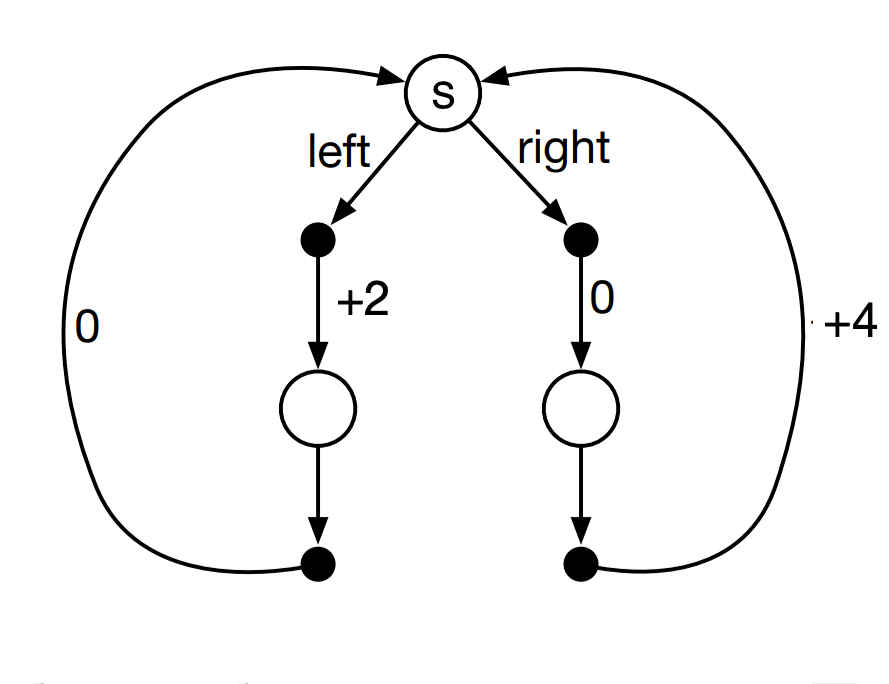
\includegraphics[width=0.6\linewidth]{figures/figure_3dot22.png}
\end{figure}
\bigspace
%\item For the above gridworld problem, draw the backup diagram for $q_{\pi}$ and $v_{\pi}$ where $\pi$ is
\begin{enumerate}
  \item a uniformly random policy
  \item a greedy policy
\end{enumerate}

\smallskip
%\item \input{questions/q_vs_v.tex}
\end{enumerate}

\end{document}
%%% Local Variables:
%%% mode: latex
%%% TeX-master: t
%%% End: